\documentclass{article}

% Language setting
% Replace `english' with e.g. `spanish' to change the document language
\usepackage[english]{babel}

% Set page size and margins
% Replace `letterpaper' with `a4paper' for UK/EU standard size
\usepackage[letterpaper,top=2cm,bottom=2cm,left=3cm,right=3cm,marginparwidth=1.75cm]{geometry}

% Useful packages
\usepackage{amsmath}
\usepackage{amssymb}
\usepackage{graphicx}
\usepackage[colorlinks=true, allcolors=blue]{hyperref}
\newtheorem{definition}{Definition}
\newtheorem{remark}{Remark}
\newtheorem{example}{Example}

\title{Differential Topology}
\author{Djordje Mihajlovic}

\begin{document}
\maketitle

\begin{abstract}
\centering
(Arduously) concise notes on Differential Topology based on lectures and lecture notes by Prof.\ Murad Alim at Heriot Watt University.
\end{abstract}

\section{Smooth Manifolds}

\subsection{The Differential.}

The goals of section one are to introduce the following concepts that will be central to differential topology; smooth manifolds, smooth maps and tangent spaces.

To begin, consider the following map:

$$f: \Re^{2} \rightarrow \Re^{3}$$

\begin{align}
        \begin{bmatrix}
           x \\
           y \\
         \end{bmatrix}
         \rightarrow
         \begin{bmatrix}
             f_{1}(x, y) \\
             f_{2} (x, y) \\
             f_{3} (x, y)
         \end{bmatrix} 
         = 
         \begin{bmatrix}
             y^{2} \\ 
             xy \\
             x^{2}
         \end{bmatrix}
\end{align}

We want to know properties of this map, specifically whether it is smooth, linear or Jacobian.

\begin{definition}
  Let $U \subset \Re^{m}$ and $V \subset \Re^{n}$ be open sets\footnote{An open set $U$ is a set in which $\forall P\in U; \exists x$ sufficiently near to P.}.
  We consider the mapping $f: U \rightarrow V$ to be smooth iff it is infinitely differentiable. That is, all partial derivatives exist and it is continuous\footnote{A map is continuous iff the preimageof any open set, is open.}\footnote{The image of $x$ is given $f(x)$ $\therefore$ the preimage of $f^{-1}(y) = \{ x| f(x) = y \}$.}.
\end{definition}

\begin{definition}
    For a smooth map
    $f = (f_{1}, f_{2}, ..., f_{n}) : U \rightarrow V$ and the point $x \in U$, the derivative is defined by the linear map $df(x): \Re^{m} \rightarrow \Re^{n}$ defined via a small movement $\eta$ where $\eta \in \Re^{m}$ such that:
    $$df(x) = \frac{f(x + t\eta) - f(x)}{t}$$
\end{definition}

Fixing the coordinates $(x_1, x_2, x_3, ..., x_n)$ the derivative is therefore defined via the Jacobian matrix:

$$df(x)_{ij} = \frac{\partial f_{i}}{\partial x^{j}}(x)$$


The differential satisfies several properties, namely:

\begin{itemize}
    \item Chain rule: \\ If $U \in \Re^{m}$, $V \in \Re^{n}, W \in \Re^{p}$ and f and g are specified smooth maps such that $f: U \rightarrow V$, $g: V \rightarrow W$ then: 
    $$d(g \circ f) (x) = dg(f(x)) \circ df(x)$$

    \item Identity: \\
    Suppose the identity mapping $id_{U}: U \rightarrow U$, this has the differential:
    $$d(id_{U}(x)) = id_{\Re^{m}}$$
\end{itemize}

\subsection{Smooth Manifolds}

\begin{definition}
        (Smooth m-Manifolds). A smooth m manifold is some space M equipped with an open cover $\{U_{\alpha}\}_{\alpha \in A}$ (i.\ e.\ some inscription over a set of points within M) and a collection of homeomorphisms $\phi_{\alpha}: U_{\alpha} \rightarrow \Omega_{\alpha}$ onto the open set $\Omega_{\alpha} \subset \Re^{m}$ (i.\ e.\ a continuous, and bijective (surjective and injective) mapping between two the two sets $U_{\alpha}$ and $\Omega_{\alpha}$). Such that, for each pair $\alpha, \beta \in A$, the transition map: $$\phi_{\beta \alpha}:= \phi_{\beta}\circ\phi_{\alpha}^{-1}:\phi_{\alpha}(U_{\alpha}\cap U_{\beta})\rightarrow \phi_{\beta}(U_{\alpha}\cap U_{\beta})$$ is smooth.
\end{definition}

% \begin{figure}
%     \centering
%     \includegraphics[width=0.5\linewidth]{frog.jpg}
%     \caption{Caption}
%     \label{fig:smooth_manifolds}
% \end{figure}

The homeomorphisms $\phi_{\alpha}$ are called `coordinate charts' and the collection $A:= \{U_{\alpha}, \phi_{\alpha}\}_{\alpha \in A}$ is called an `atlas'.

\begin{figure}[hbt!]
    \centering
    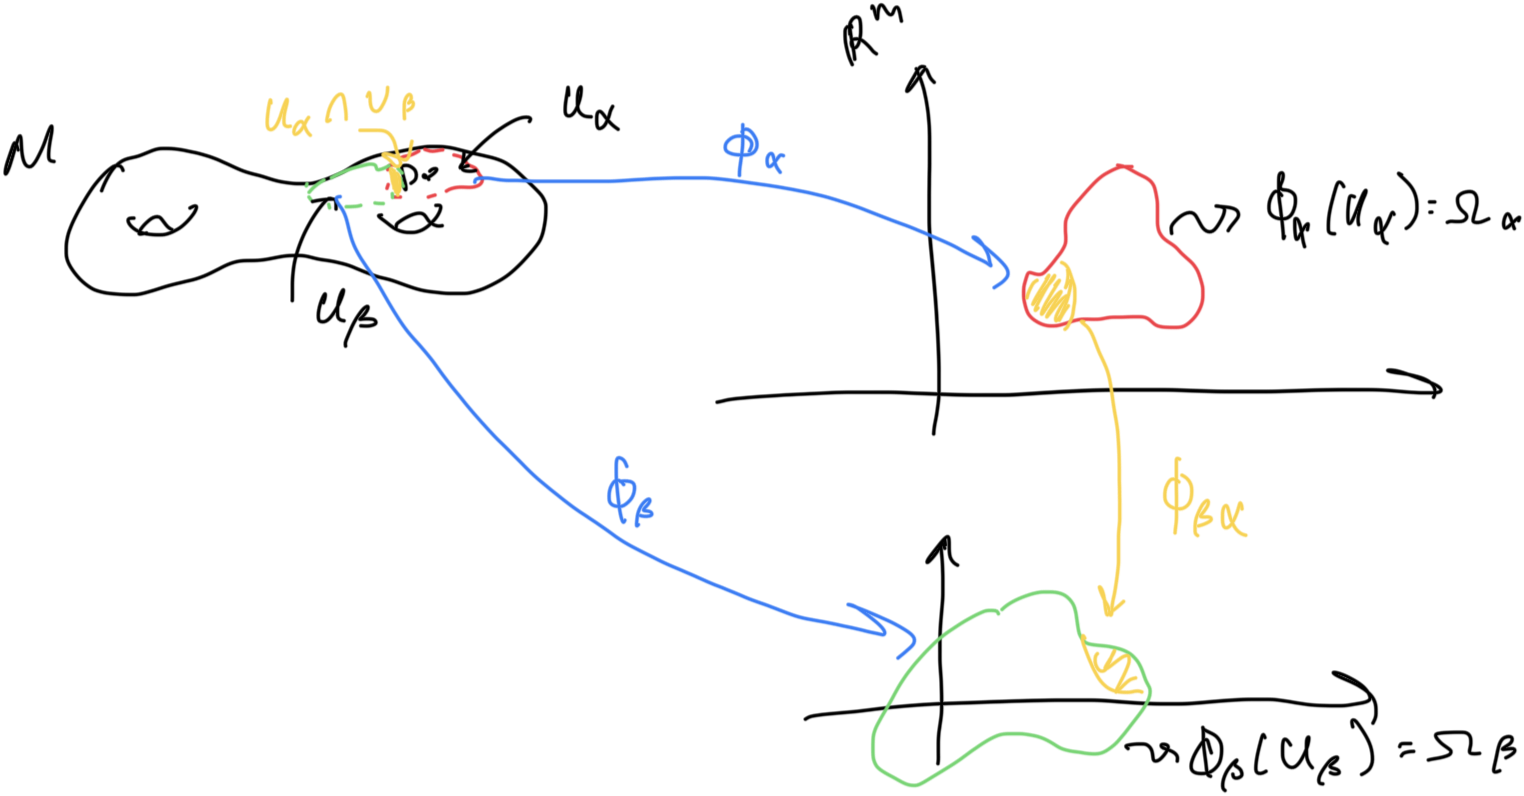
\includegraphics[width=0.6\linewidth]{figures/coordinate_charts_1.PNG}
    \caption{A smooth manifold $M$ with open sets $U_{\alpha}$ and $U_{\beta}$ shown along with their coordinate charts and subsequent interpretation of the transition map $\phi_{\beta \alpha}$}
    \label{fig:coordinate_chart}
\end{figure}

\begin{remark}
        Compatibility: A homeomorphism $\phi_{c}: U_{c} \rightarrow \Omega_{c}$ from the open subset $U_{c}\subset M$ to $\Omega_{c}\subset \Re^{m}$ is compatible with atlas $A:=\{U_{\alpha}, \phi_{\alpha}\}_{\alpha \in A}$ iff: $$\phi_{\alpha}\circ \phi_{c}^{-1}: \phi_{c}(U_{c}\cap U_{\alpha}) \rightarrow \phi_{\alpha}(U_{c} \cap U_{\alpha})$$
        is a diffeomorphism\footnote{An isomorphism of differentiable manifolds; that is, it is a mapping that is structure preserving and has an inverse.} for all $\alpha$.
        \begin{figure}[hbt!]
            \centering
            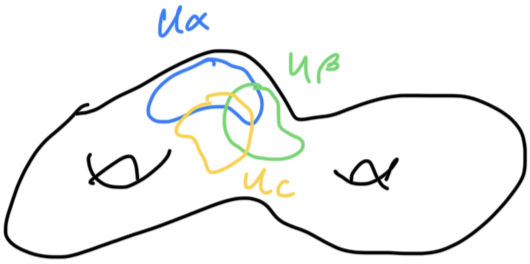
\includegraphics[width=0.3\linewidth]{figures/compatiblity_atlas.PNG}
            \caption{If $U_{\alpha}$ and $U_{\beta}$ equipped with the coordinate charts $\phi_{\alpha}$ and $\phi_{\beta}$ are in the atlas $A$ then the homeomorphism $\phi_{c}$ for open set $U_{c}$ must satisfy the diffeomorphism condition for its intersections with $U_{\alpha}$ and $U_{\beta}$.}
            \label{fig:compatibility}
        \end{figure}
\end{remark}
\begin{remark}
        Smooth structure: An atlas $A$ is called maximal if it contains every coordinate chart that is compatible with all its members.
\end{remark}

\begin{example}
    
\end{example}

\subsection{Smooth Maps}

Define two m and n-manifolds $M$ and $N$ along with their corresponding atlases as: $(M, \{ \phi_{\alpha}, U_{\alpha} \}_{\alpha \in A})$ and $(N, \{ \psi_{\beta}, U_{\beta} \} _{\beta \in B})$. 

\begin{definition}
        Smooth maps:
        A map $f: M \rightarrow N$ is called smooth if it is continuous and the map $f_{\beta, \alpha}$ is smooth for $\forall \alpha \in A, \beta \in B$. 
        \begin{figure}[hbt!]
            \centering
            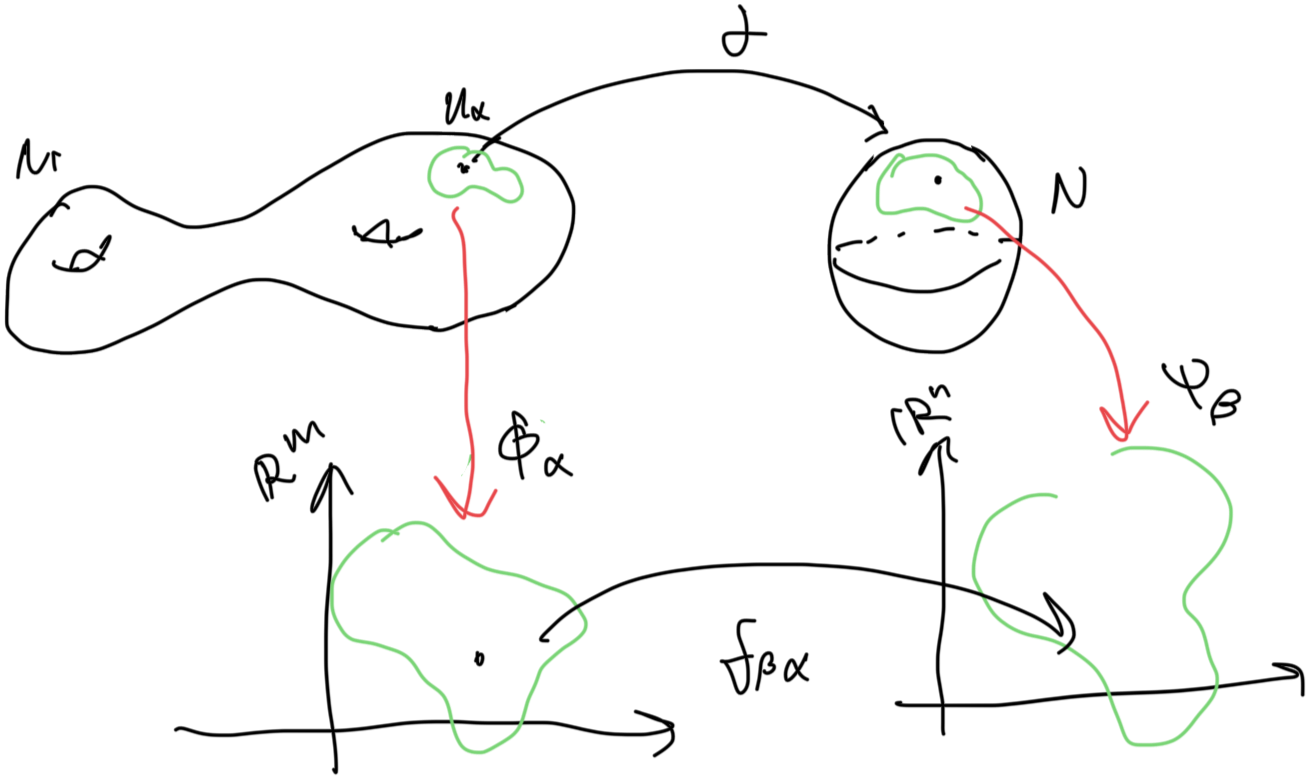
\includegraphics[width=0.5\linewidth]{figures/smooth_map.PNG}
            \caption{The smooth map between the manifolds m and n.}
            \label{fig:smooth_maps}
        \end{figure}
\end{definition}

\begin{example}
        Example
\end{example}

\subsection{Tangent Spaces}

\begin{definition}
        Suppose the manifold $M$ equipped with an atlas $A$ such that we have the usual representation. We can therefore define the tangent space of $M$ at a point $p$ as the following quotient space\footnote{Lets decompose this to make the concept more concrete, firstly the idea of a quotient space. Consider a space $X$, there are equivalence classes between some $x \in X$, where an equivalence relation is given $\sim$. we can $\therefore$ construct the \emph{set} of different equivalence classes of $X$ via $Y = X/\sim$, this is the canonical topological quotient space. Hence the tangent space of a manifold is defined in the equation as the cross product between the set of the union of points $\alpha$ in the open set $U_{\alpha}$, and the set $\Re^{m}$ modulo the equivalence relations of the point $p$, $\sim^{p}$, leaving us with the set of different equivalence classes of the cross product between the union of open sets $\bigcup_{p\in U_{\alpha}}$ and $\Re^{m}$.}: $$T_{p}M := \bigcup_{p\in U_{\alpha}}\{\alpha \} \times  \Re^{m}/\sim^{p}$$
        where the union can be understood as the collection of all $\alpha \in A$ with $p \in U_{\alpha}$ and\footnote{This is how the equivalence relation $\sim^{p}$ is defined. In particular, it is saying that the pair $(\alpha, \xi)$ is equivalent to $(\beta, \eta)$ if there is a  mapping between the derivatives of coordinate charts.}
        $$(\alpha, \xi) \sim^{p} (\beta, \eta) \rightleftharpoons d(\phi_{b} \circ \phi_{\alpha}^{-1})(x)\xi = \eta, x:= \phi_{\alpha}(p).$$
\end{definition}

\begin{figure}[hbt!]
    \centering
    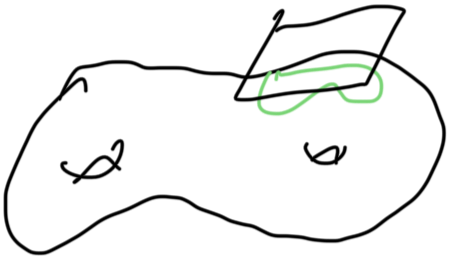
\includegraphics[width=0.3\linewidth]{figures/tangent_space.PNG}
    \caption{An example tangent space for the 2-genus, 2-manifold at some point within an open set (indicated via the green boundary).}
    \label{fig:enter-label}
\end{figure}

\begin{definition}
    The union of all tangent spaces of some manifold $M$ is known as the tangent bundle of $M$ denoted $TM$.
    $$TM := \bigcup_{p\in M}T_{p}M$$
\end{definition}

\begin{definition}
    Consider again our smooth m-manifold $M$ and smooth n-manifold $N$. Let $f$ be the smooth map between $M$ and $N$, such that $f:M\rightarrow N$. We can define the derivative of $f$ at some point $p\in M$ via the linear map: 
    $$df(p): T_{p}M\rightarrow T_{f(p)}N$$
    which is explicitly defined by
    $$f_{*}(p):= df_{p}:=df(p)[\alpha, \xi]_{p}:= [\beta, df_{\beta \alpha}(\phi_{\alpha}(p))\xi]_{f(p)}$$
\end{definition}

\begin{remark}
    Consider $N=\Re^{n}$ as a manifold with the single coordinate chart $\psi_{\beta} = id: \Re^{n}\rightarrow \Re^{n}.$ We subsequently can say that the tangent space $T_{q}N$ is isomorphic to $\Re^{n} \forall q \in N$.
    Therefore, the derivative of the smooth map $f:M \rightarrow \Re^{n}$ at $p \in M$ is a linear map $df(p): T_{p}M\rightarrow \Re^{n}$. 
    $$df(p)[\alpha, \xi]_{p} = d(f \circ \phi^{-1}_{\alpha})(x)\xi$$ with $p \in U_{\alpha}$, $x:= \phi_{\alpha}(p)$ and $\xi \in \Re^{m}$
    \begin{figure}[hbt!]
        \centering
        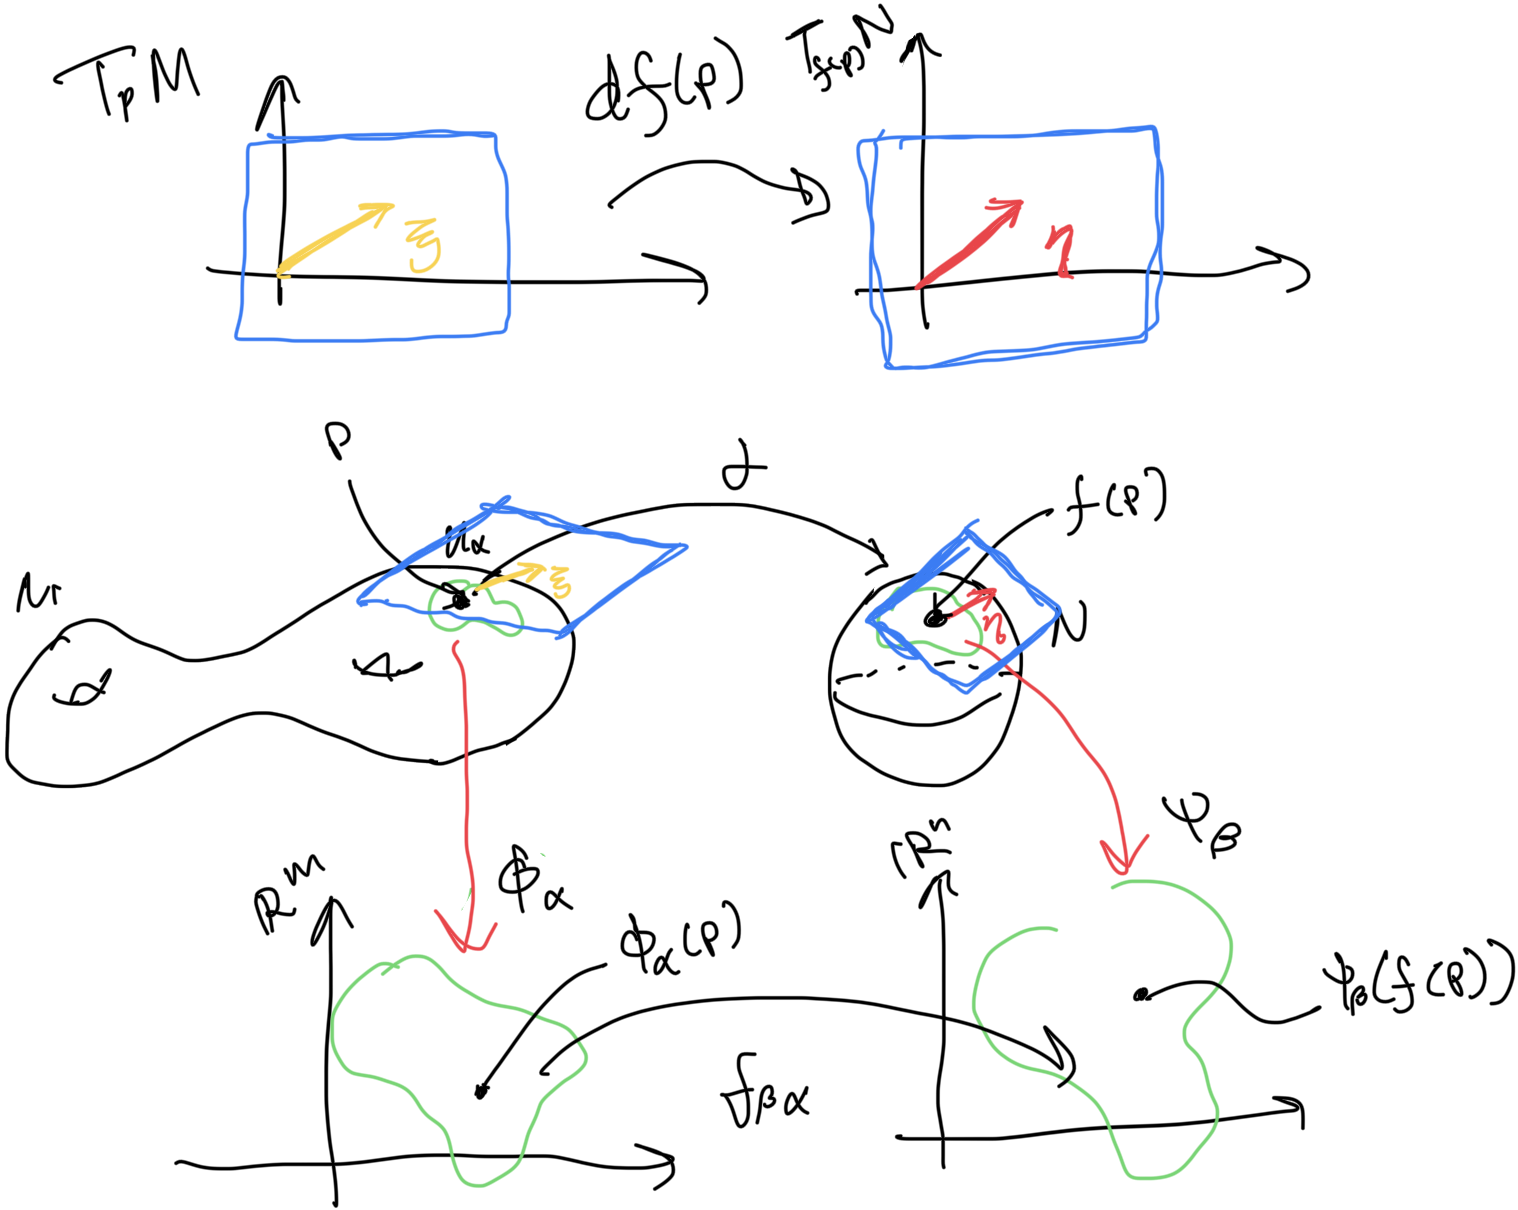
\includegraphics[width=0.65\linewidth]{figures/derivative_of_smooth_maps.PNG}
        \caption{Derivative ($df(p)$) of the smooth mapping $f$ between manifolds $M$ and $N$.}
        \label{fig:derivative_smooth_map}
    \end{figure}
\end{remark}

\begin{example}
    Examples
\end{example}



\bibliographystyle{alpha}
\bibliography{references}

\end{document}